\chapter{Fourier Series and Signals}\index{Fourier series}

A piano and a violin can play the same note, at the same loudness, and you can
still tell them apart with your eyes closed. In the Sound chapter, you learned
why: each instrument adds its own mix of overtones to the fundamental frequency.
In 1807, Joseph Fourier made a much bolder claim. \emph{Every} repeating signal,
no matter how jagged, can be built by adding up sine and cosine waves. A square
wave, a heartbeat, the hum of a refrigerator: all of them are sums of pure tones.

Fourier's idea now runs inside almost every device you own. Your phone uses it to
compress music, your earbuds use it to cancel noise, and your speakers use it to
send each sound to the right driver. This chapter shows how to find the recipe of
sines inside a signal, and what you can do once you have it.

\section{Building a Wave from Sines}\index{square wave}
Start with a square wave: a signal that jumps between $-1$ and $1$, like a switch
flipping on and off. It is about as far from a smooth sine wave as a signal can
be. Yet look at what happens when we add these sine waves:
$$\frac{4}{\pi}\left(\sin x + \frac{\sin 3x}{3} + \frac{\sin 5x}{5} + \frac{\sin 7x}{7} + \cdots\right)$$

\begin{minted}{python}
import numpy as np
import matplotlib.pyplot as plt

x = np.linspace(-np.pi, np.pi, 1000)

def partial_sum(x, terms):
    """The first `terms` nonzero terms of the square wave's Fourier series."""
    total = np.zeros_like(x)
    for k in range(terms):
        n = 2 * k + 1                    # only odd n appear
        total += 4 / (n * np.pi) * np.sin(n * x)
    return total

plt.plot(x, np.sign(x), "k", linewidth=2, label="square wave")
for terms in [1, 3, 15]:
    plt.plot(x, partial_sum(x, terms), label=f"{terms} term" + ("s" if terms > 1 else ""))
plt.xlabel("x")
plt.legend()
plt.savefig("square_wave.png")
\end{minted}

\begin{figure}[H]
\centering
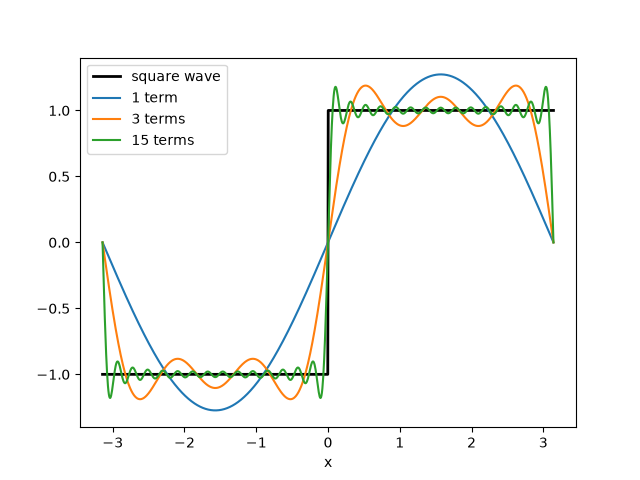
\includegraphics[width=0.7\textwidth]{square_wave.png}
\caption{Adding more sine waves brings the sum closer and closer to a square wave.}
\label{fig:square-wave}
\end{figure}

One sine wave is a rough sketch. Three already have the flat top and the steep
sides. Fifteen hug the square wave almost everywhere. Where did the numbers
$\frac{4}{\pi}$, $\frac{1}{3}$, $\frac{1}{5}$, $\dots$ come from? That is what the rest of
this section is about.

\subsection{Fourier Series}
A function $f$ is \newterm{periodic} with period $2\pi$ if $f(x + 2\pi) = f(x)$ for
every $x$. Its \newterm{Fourier series} is
$$f(x) = \frac{a_0}{2} + \sum_{n=1}^{\infty} \left(a_n\cos nx + b_n\sin nx\right)$$
The numbers $a_n$ and $b_n$ are the \newterm{Fourier coefficients}. They say how
much of each frequency is in the signal: $b_3$, for example, is the amount of the
wave $\sin 3x$, which wiggles three times as fast as $\sin x$.

\subsection{The Key Fact: Orthogonality}\index{orthogonality}
Finding the coefficients rests on one fact about integrals. For positive whole
numbers $m$ and $n$,
$$\int_{-\pi}^{\pi} \sin mx \,\sin nx\,dx = \begin{cases} 0 & m \neq n \\ \pi & m = n\end{cases}$$
The same is true with both sines replaced by cosines, and
$\int_{-\pi}^{\pi} \sin mx\,\cos nx\,dx = 0$ always.

To see why, subtract the two sum formulas from the Trigonometric Identities
chapter, $\cos(A - B) - \cos(A + B) = 2\sin A\sin B$. So
$$\sin mx\,\sin nx = \frac{1}{2}\left[\cos\big((m - n)x\big) - \cos\big((m + n)x\big)\right]$$
For any nonzero whole number $k$, $\int_{-\pi}^{\pi}\cos kx\,dx = \left[\frac{\sin kx}{k}\right]_{-\pi}^{\pi} = 0$,
because $\sin$ is zero at every multiple of $\pi$. When $m \neq n$, both cosines have
a nonzero $k$, so the integral is 0. When $m = n$, the first cosine is
$\cos 0 = 1$, and the integral is $\frac{1}{2}(2\pi) = \pi$. Finally, $\sin mx\cos nx$
is an odd function, so its integral over a symmetric interval is 0.

Sines and cosines of different frequencies ``cancel out'' when you multiply them
and integrate, the same way perpendicular vectors have a dot product of zero. That
is why mathematicians call them \newterm{orthogonal}.

\subsection{Finding the Coefficients}
Multiply both sides of the Fourier series by $\sin mx$ and integrate from $-\pi$ to
$\pi$. By orthogonality, every term on the right vanishes except one, $b_m\pi$. The
same trick with $\cos mx$ picks out $a_m$:

\begin{mdframed}[style = important, frametitle = {Fourier Coefficients}]
$$a_n = \frac{1}{\pi}\int_{-\pi}^{\pi} f(x)\cos nx\,dx, \qquad b_n = \frac{1}{\pi}\int_{-\pi}^{\pi} f(x)\sin nx\,dx$$
\end{mdframed}

Each integral measures how much $f$ ``looks like'' one particular wave: it is large
when $f$ rises and falls in step with that wave and zero when they have nothing in
common.

\textbf{Example}: Find the Fourier series of the square wave $f(x) = -1$ for
$-\pi < x < 0$ and $f(x) = 1$ for $0 < x < \pi$.

\textbf{Solution}: The square wave is an odd function, and $\cos nx$ is even, so
$f(x)\cos nx$ is odd and every $a_n = 0$. For $b_n$, the two halves contribute
equally:
$$b_n = \frac{1}{\pi}\left(\int_{-\pi}^{0} -\sin nx\,dx + \int_{0}^{\pi} \sin nx\,dx\right) = \frac{2}{\pi}\int_0^\pi \sin nx\,dx = \frac{2}{\pi}\cdot\frac{1 - \cos n\pi}{n}$$
Since $\cos n\pi$ is $-1$ for odd $n$ and $1$ for even $n$, $b_n = \frac{4}{n\pi}$ when
$n$ is odd and $b_n = 0$ when $n$ is even. That is exactly the recipe in the
program above.

\subsection{A Surprise Bonus}
Set $x = \frac{\pi}{2}$, where the square wave equals 1. Since
$\sin\frac{\pi}{2} = 1$, $\sin\frac{3\pi}{2} = -1$, $\sin\frac{5\pi}{2} = 1$, and so on,
$$1 = \frac{4}{\pi}\left(1 - \frac{1}{3} + \frac{1}{5} - \frac{1}{7} + \cdots\right) \quad\Longrightarrow\quad \frac{\pi}{4} = 1 - \frac{1}{3} + \frac{1}{5} - \frac{1}{7} + \cdots$$
That is the series for $\arctan 1$ from the Taylor and Maclaurin Series chapter,
reached by a completely different road.

\subsection{The Gibbs Phenomenon}\index{Gibbs phenomenon}
Look closely at figure \ref{fig:square-wave}: next to each jump, the partial sums
overshoot. You might expect the overshoot to fade as you add terms. It does not.
It gets narrower, but its peak stays near $1.179$, about 9\% of the jump, no
matter how many terms you use. This is the \newterm{Gibbs phenomenon}. Engineers
hear it as ``ringing'' when a sharp-edged signal passes through equipment that
cuts off high frequencies.

\begin{Exercise}[title={Orthogonality by Hand}, label=fs_orth]
Use the identity $\sin A\sin B = \frac{1}{2}[\cos(A - B) - \cos(A + B)]$ to show that
$\int_{-\pi}^{\pi}\sin 2x\,\sin 3x\,dx = 0$.
\end{Exercise}
\begin{Answer}[ref=fs_orth]
$\sin 2x\sin 3x = \frac{1}{2}[\cos(-x) - \cos 5x] = \frac{1}{2}[\cos x - \cos 5x]$. Then
$$\int_{-\pi}^{\pi} \frac{1}{2}(\cos x - \cos 5x)\,dx = \frac{1}{2}\left[\sin x - \frac{\sin 5x}{5}\right]_{-\pi}^{\pi} = 0$$
because $\sin$ is 0 at $\pm\pi$ and $\pm 5\pi$.
\end{Answer}

\begin{Exercise}[title={The Sawtooth Wave}, label=fs_saw]
The sawtooth wave is $f(x) = x$ for $-\pi < x < \pi$, repeated every $2\pi$. Find its
Fourier coefficients. (Hint: integrate by parts.)
\end{Exercise}
\begin{Answer}[ref=fs_saw]
The function is odd, so every $a_n = 0$. By parts, with $u = x$ and $dv = \sin nx\,dx$,
$$b_n = \frac{1}{\pi}\int_{-\pi}^{\pi} x\sin nx\,dx = \frac{1}{\pi}\left[-\frac{x\cos nx}{n}\right]_{-\pi}^{\pi} + \frac{1}{\pi n}\int_{-\pi}^{\pi}\cos nx\,dx = -\frac{2\cos n\pi}{n} + 0 = \frac{2(-1)^{n+1}}{n}$$
So $x = 2\left(\sin x - \frac{\sin 2x}{2} + \frac{\sin 3x}{3} - \cdots\right)$. Unlike the
square wave, the sawtooth contains every harmonic, not just the odd ones.
\end{Answer}

\begin{Exercise}[title={Three Terms}, label=fs_three]
Evaluate the first three nonzero terms of the square wave's series at $x = \frac{\pi}{2}$.
Is the result above or below 1? Use figure \ref{fig:square-wave} to explain.
\end{Exercise}
\begin{Answer}[ref=fs_three]
$\frac{4}{\pi}\left(1 - \frac{1}{3} + \frac{1}{5}\right) \approx 1.1035$, which is above 1. In the
figure, the 3-term curve wiggles above and below the flat top, and $x = \frac{\pi}{2}$
is at one of its peaks. Adding more terms makes the wiggles smaller.
\end{Answer}

\section{Frequencies, Harmonics, and Timbre}\index{harmonics}
Real signals do not have a period of $2\pi$. A note with frequency $f_1$ repeats every
$T = \frac{1}{f_1}$ seconds, and its Fourier series becomes
$$s(t) = \frac{a_0}{2} + \sum_{n=1}^{\infty}\left(a_n\cos(2\pi n f_1 t) + b_n\sin(2\pi n f_1 t)\right)$$
Every term is a pure tone at a whole-number multiple of the \newterm{fundamental
frequency} $f_1$: the \newterm{harmonics} $f_1, 2f_1, 3f_1, \dots$. These are the
overtones from the Sound chapter, and the coefficients are the recipe. An
instrument's \newterm{timbre}, the quality that makes a violin sound like a violin,
is the pattern of sizes of its Fourier coefficients.

A square wave contains only odd harmonics, which gives it a hollow, reedy sound,
a bit like a clarinet. A sawtooth contains all of them and sounds bright and
buzzy, which is why it is a favorite starting point for synthesizers.

\subsection{The Complex Form}
With Euler's formula from the previous chapter, $\cos$ and $\sin$ combine into one
exponential, and the series becomes shorter:
$$f(x) = \sum_{n=-\infty}^{\infty} c_n e^{inx}, \qquad c_n = \frac{1}{2\pi}\int_{-\pi}^{\pi} f(x)e^{-inx}\,dx$$
Each $e^{inx}$ is a point spinning around the unit circle $n$ times per period, and
$c_n$ is a complex number whose size is the amplitude and whose angle is the phase
(how far the wave is shifted). Engineers and physicists almost always use this form.

\begin{Exercise}[title={Harmonics of a Square Wave}, label=fs_harm]
An electronic keyboard plays a square-wave tone at 220 Hz. List the frequencies and
relative amplitudes of its first four nonzero harmonics.
\end{Exercise}
\begin{Answer}[ref=fs_harm]
Only odd harmonics appear, with amplitudes proportional to $\frac{1}{n}$: 220 Hz
(amplitude 1), 660 Hz ($\frac{1}{3}$), 1100 Hz ($\frac{1}{5}$), and 1540 Hz ($\frac{1}{7}$).
\end{Answer}

\section{Sampled Signals and the FFT}\index{discrete Fourier transform}\index{FFT}
A microphone does not hand a computer a formula. Digital audio stores
\newterm{samples}: the height of the wave measured thousands of times per second. The
\newterm{discrete Fourier transform} (DFT) does for a list of samples what the
integrals did for a function: it finds the amplitude of each frequency. A clever way
of computing it, the \newterm{fast Fourier transform} (FFT), made it practical; it is
one of the most important algorithms ever written.

Here is a one-second signal made of a 440 Hz note (the A above middle C) and two
overtones. The FFT pulls the recipe back out:
\begin{minted}{python}
import numpy as np
import matplotlib.pyplot as plt

rate = 8000                          # samples per second
t = np.arange(0, 1, 1 / rate)        # one second of time

# A 440 Hz note with two overtones
signal = (1.0 * np.sin(2 * np.pi * 440 * t)
          + 0.5 * np.sin(2 * np.pi * 880 * t)
          + 0.25 * np.sin(2 * np.pi * 1320 * t))

spectrum = np.abs(np.fft.rfft(signal)) / (len(t) / 2)   # amplitudes
freqs = np.fft.rfftfreq(len(t), 1 / rate)               # in Hz

for f, a in zip(freqs, spectrum):
    if a > 0.1:
        print(f"{f:.0f} Hz: amplitude {a:.2f}")

fig, (top, bottom) = plt.subplots(2, 1)
top.plot(t[:160] * 1000, signal[:160])
top.set_xlabel("time (ms)")
bottom.plot(freqs, spectrum)
bottom.set_xlim(0, 2000)
bottom.set_xlabel("frequency (Hz)")
fig.tight_layout()
fig.savefig("spectrum.png")
\end{minted}
\begin{verbatim}
440 Hz: amplitude 1.00
880 Hz: amplitude 0.50
1320 Hz: amplitude 0.25
\end{verbatim}

\begin{figure}[H]
\centering
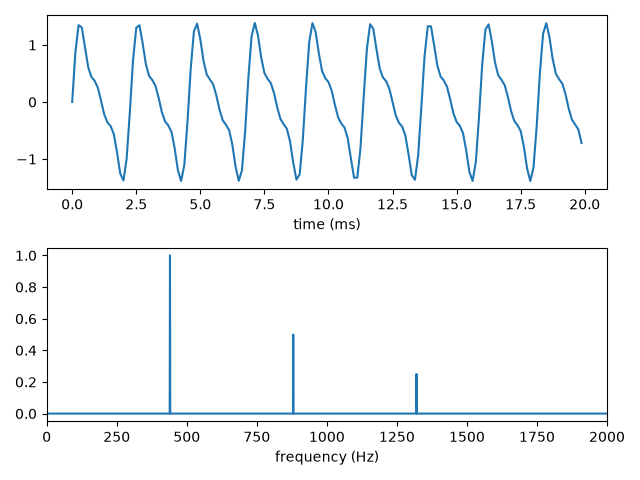
\includegraphics[width=0.75\textwidth]{spectrum.png}
\caption{Top: 20 ms of the signal, a lopsided wave. Bottom: its
\newterm{spectrum}, three spikes at the three frequencies inside it.}
\label{fig:spectrum}
\end{figure}

The top picture is hard to read; the bottom one tells you everything. Viewing a
signal as a \emph{spectrum}, amplitude against frequency, is often far more useful
than viewing it against time.

\subsection{How Fast Must You Sample?}\index{Nyquist frequency}
To capture a wave, you need more than two samples per cycle. A wave sampled too
slowly is mistaken for a slower one, an effect called \newterm{aliasing} (it is why
car wheels sometimes seem to spin backward in videos). So a sampling rate of $r$
samples per second can only represent frequencies below $\frac{r}{2}$, the
\newterm{Nyquist frequency}. CDs sample at 44,100 Hz, so they can hold frequencies up
to 22,050 Hz, just above the roughly 20,000 Hz limit of human hearing.

\begin{Exercise}[title={Sampling Rates}, label=fs_nyq]
A phone records audio at 48,000 samples per second. What is the highest frequency it
can capture? Could it record the 40,000 Hz call of a bat?
\end{Exercise}
\begin{Answer}[ref=fs_nyq]
The Nyquist frequency is $\frac{48{,}000}{2} = 24{,}000$ Hz. A 40,000 Hz call is above
that, so the phone cannot record it. (It would show up, if at all, as an alias at a
false, lower frequency.)
\end{Answer}

\section{Filters and Speaker Crossovers}\index{filter}\index{speaker crossover}
Once a signal is a sum of frequencies, changing its sound is simple: turn some
frequencies up and others down. A device that does this is a \newterm{filter}. A
\newterm{low-pass} filter lets low frequencies through and weakens high ones; a
\newterm{high-pass} filter does the opposite. The bass and treble knobs on a stereo
are filters, and so is a graphic equalizer, which has a slider for each band of
frequencies.

\subsection{Why Speakers Need Crossovers}
No single speaker cone is good at everything. To make deep bass, a speaker must
push a lot of air, so it needs a big, heavy cone, called a \newterm{woofer}. But a heavy
cone cannot shake back and forth 10,000 times a second. High notes need a small, light
cone, a \newterm{tweeter}, and feeding a tweeter strong bass can tear it apart. So most
speakers contain both, plus a \newterm{crossover}: a pair of filters that sends the
low frequencies to the woofer and the high frequencies to the tweeter.

The simplest crossover uses just two parts, using the reactances from the Pendulums
and Alternating Current chapter:
\begin{itemize}
\item A \textbf{capacitor} in series with the tweeter. Its reactance,
$X_C = \frac{1}{2\pi fC}$, is huge at low frequencies, so it blocks the bass and lets
the treble through: a high-pass filter.
\item An \textbf{inductor} in series with the woofer. Its reactance, $X_L = 2\pi fL$, is
huge at high frequencies, so it blocks the treble: a low-pass filter.
\end{itemize}
The handoff happens at the \newterm{crossover frequency} $f_c$, where the part's
reactance equals the speaker's resistance $R$:
$$f_c = \frac{1}{2\pi RC} \quad\text{(tweeter)}, \qquad f_c = \frac{R}{2\pi L} \quad\text{(woofer)}$$
For these first-order filters, the fraction of the signal each speaker receives at
frequency $f$ is
$$\text{woofer: } \frac{1}{\sqrt{1 + (f/f_c)^2}}, \qquad \text{tweeter: } \frac{f/f_c}{\sqrt{1 + (f/f_c)^2}}$$

\textbf{Example}: Design a crossover at 2500 Hz for 8 $\Omega$ speakers.

\textbf{Solution}: For the tweeter,
$C = \frac{1}{2\pi(8)(2500)} \approx 7.96 \times 10^{-6}$ F, about $8\ \mu$F. For the woofer,
$L = \frac{8}{2\pi(2500)} \approx 0.51 \times 10^{-3}$ H, about $0.51$ mH. Check the capacitor:
at 100 Hz its reactance is about $199\ \Omega$, far more than the tweeter's $8\ \Omega$, so
bass is blocked; at 10,000 Hz it is only about $2\ \Omega$.

\begin{minted}{python}
import numpy as np
import matplotlib.pyplot as plt

fc = 2500                                  # crossover frequency, Hz
f = np.logspace(1, np.log10(20000), 500)   # 10 Hz to 20 kHz

woofer = 1 / np.sqrt(1 + (f / fc) ** 2)               # low-pass
tweeter = (f / fc) / np.sqrt(1 + (f / fc) ** 2)       # high-pass

for test in [100, 2500, 10000]:
    w = 1 / np.sqrt(1 + (test / fc) ** 2)
    tw = (test / fc) / np.sqrt(1 + (test / fc) ** 2)
    print(f"{test} Hz: woofer {w:.2f}, tweeter {tw:.2f}")

plt.semilogx(f, woofer, label="woofer (low-pass)")
plt.semilogx(f, tweeter, label="tweeter (high-pass)")
plt.axvline(fc, color="gray", linestyle="--")
plt.xlabel("frequency (Hz)")
plt.ylabel("fraction of the signal passed")
plt.legend()
plt.savefig("crossover.png")
\end{minted}
\begin{verbatim}
100 Hz: woofer 1.00, tweeter 0.04
2500 Hz: woofer 0.71, tweeter 0.71
10000 Hz: woofer 0.24, tweeter 0.97
\end{verbatim}

\begin{figure}[H]
\centering
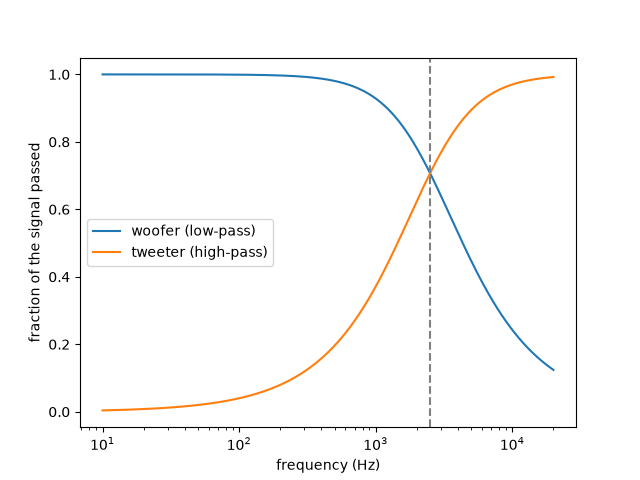
\includegraphics[width=0.7\textwidth]{crossover.png}
\caption{A first-order crossover at 2500 Hz. Bass goes to the woofer, treble to the
tweeter, and both share the frequencies near $f_c$.}
\label{fig:crossover}
\end{figure}

At the crossover frequency, each speaker gets $\frac{1}{\sqrt{2}} \approx 0.71$ of the
signal, and therefore half the power (power goes as the square). In fact, at
\emph{every} frequency, the squares of the two fractions add to exactly 1:
$\frac{1}{1 + u^2} + \frac{u^2}{1 + u^2} = 1$ with $u = f/f_c$. The total power
reaching the two speakers stays the same; the crossover only decides who gets it.
Real speakers often use steeper, higher-order crossovers, and many powered speakers
now do the job digitally, with an FFT-style filter running on a chip.

\begin{Exercise}[title={Design a Crossover}, label=fs_xover]
Design a first-order crossover at 3000 Hz for 4 $\Omega$ speakers. What capacitor
goes with the tweeter, and what inductor goes with the woofer?
\end{Exercise}
\begin{Answer}[ref=fs_xover]
$C = \frac{1}{2\pi(4)(3000)} \approx 13.3\ \mu$F and $L = \frac{4}{2\pi(3000)} \approx 0.212$ mH.
\end{Answer}

\begin{Exercise}[title={Filtering a Square Wave}, label=fs_filter]
A 440 Hz square-wave tone passes through a first-order low-pass filter with
$f_c = 1000$ Hz. What fraction of each of the first four harmonics gets through? How
will the tone sound different?
\end{Exercise}
\begin{Answer}[ref=fs_filter]
The harmonics are at 440, 1320, 2200, and 3080 Hz. Using
$\frac{1}{\sqrt{1 + (f/1000)^2}}$, the fractions are about 0.92, 0.60, 0.41, and 0.31.
The fundamental passes almost untouched, but the higher harmonics are cut more and
more, so the corners of the square wave round off and the tone sounds softer and
more muffled, closer to a pure sine wave.
\end{Answer}

\begin{Exercise}[title={Add a Tone}, label=fs_python]
Change \filename{spectrum.py} to add a fourth tone at 1760 Hz with amplitude 0.3.
What does the program print now?
\end{Exercise}
\begin{Answer}[ref=fs_python]
Add \mintinline{python}{+ 0.3 * np.sin(2 * np.pi * 1760 * t)} to the signal. The program
then prints a fourth line, \texttt{1760 Hz: amplitude 0.30}, after the other three.
\end{Answer}
